% Foliensatz: "AFu-Kurs nach DJ4UF" von DK0TU, Amateurfunkgruppe der TU Berlin
% Lizenz: CC BY-NC-SA 3.0 de (http://creativecommons.org/licenses/by-nc-sa/3.0/de/)
% Autoren: Martin Deutschmann, Lars Weiler <dc4lw@darc.de>, Felix Baum <baumfelix@gmail.com>

\documentclass[aspectratio=169]{beamer}

\usepackage[ngerman]{babel} % deutsche Worttrennung etc.
\usepackage[utf8]{inputenc} % UTF8 Text

\usepackage[super, comma, numbers, square, sort]{natbib}

\usepackage{hyperref}       % Hyperref Package für bessere Referenzen (todo)
\hypersetup{
	colorlinks=false,       %   false: boxed links; true: colored links
    %linkcolor=white,       %   color of internal links (change box color with linkbordercolor)
    citecolor=red,          %   color of links to bibliography
    filecolor=white,        %   color of file links
    urlcolor=blue           %   color of external links
}

\usepackage{multirow}
\usepackage{wasysym}  % Math Symbols like \permil
%\usepackage{colortbl}
%\usepackage{subscript}
%\usepackage{caption}
%\usepackage{setspace}
%\usepackage{xcolor}        % benutze CodeListe

% Footnote
%\usepackage{hanging}
%
%\setbeamertemplate{footnote}{%
%  \hangpara{2em}{1}%
%  \makebox[2em][l]{\insertfootnotemark}\footnotesize\insertfootnotetext\par%
%}


%\usepackage{pgf}
%\usepackage{tikz}
%\usetikzlibrary{arrows,automata}
%\usetikzlibrary{positioning}
%
%\tikzset{
%    state/.style={
%           rectangle,
%           rounded corners,
%           draw=black, very thick,
%           minimum height=2em,
%           minimum width=2pt,
%           inner sep=2pt,
%           text centered,
%           },
%}

%\usepackage{listings}
%\lstset{basicstyle=\small, numberstyle=\tiny, extendedchars=true, numbers=left, numbersep=5pt}
%\lstset{showtabs=false, showspaces=false, showstringspaces=false}
%%\lstset{backgroundcolor=\color{white!75!lightgray}, , frame=single}
%%\lstset{backgroundcolor=\color{white}}
%%\lstset{backgroundcolor=none}
%\lstset{keywordstyle=\color{blue!50!gray},  identifierstyle=\color{black}}
%\lstset{commentstyle=\color{green!50!gray}, stringstyle=\color{red!50!gray}}
%\lstset{language=C, fontadjust=true, tabsize=2, breaklines=true}
%\lstset{backgroundcolor=\color{white!75!lightgray}, caption=\lstname, frame=single}
%\lstset{emphstyle=\color{black}\fbox}
%
%% Keine "Listing:"-Caption
%\captionsetup{labelformat=empty,labelsep=none}
%
%% für mathematische Umgebungen
%\usepackage{amsmath,amsfonts,amssymb}
%
%\lstdefinestyle{Bash}{
%language=Bash,
%frame=single,
%rulecolor=\color{black},
%backgroundcolor=\color{gray!50},
%keywordstyle=\color{black},
%identifierstyle=,
%commentstyle=\color{black},
%stringstyle=\color{magenta!65!white},
%showstringspaces=false,
%basicstyle=\footnotesize\ttfamily\color{black},
%numbers=none,
%breaklines=true,
%captionpos=b
%}

%\usepackage{listings}
%
%\lstdefinestyle{basic}{
%    captionpos=t,%
%    basicstyle=\footnotesize\ttfamily,%
%    numberstyle=\tiny,%
%    numbers=left,%
%    stepnumber=1,%
%    frame=single,%
%    showspaces=false,%
%    showstringspaces=false,%
%    showtabs=false,%
%    %
%    keywordstyle=\color{blue},%
%    identifierstyle=,%
%    commentstyle=\color{gray},%
%    stringstyle=\color{magenta}%
%}



% fließende Boxen haben keinen Abstand
%\fboxsep0mm

% inkludiere Creative Commons Helper
%%%%%%%%%%%%%%%%%%%%%%%%%%%%%%%%%%%%%%%%%%%%%%%%%%%%%%%%%%%%%%%%
%% ccBeamer 0.1, 2007-07-02                                   %%
%% Written by Sebastian Pipping <webmaster@hartwork.org>      %%
%% ---------------------------------------------------------- %%
%% Licensed under Creative Commons Attribution-ShareAlike 3.0 %%
%% http://creativecommons.org/licenses/by-sa/3.0/             %%
%%%%%%%%%%%%%%%%%%%%%%%%%%%%%%%%%%%%%%%%%%%%%%%%%%%%%%%%%%%%%%%%


%% Images
\newcommand{\CcImageBy}[1]{%
	
\includegraphics[scale=#1]{texdata/creative_commons/cc_by_30.pdf}%
}
\newcommand{\CcImageCc}[1]{%
	
\includegraphics[scale=#1]{texdata/creative_commons/cc_cc_30.pdf}%
}
\newcommand{\CcImageDevNations}[1]{%
	
\includegraphics[scale=#1]{texdata/creative_commons/cc_dev_nations_30.pdf}%
}
\newcommand{\CcImageNc}[1]{%
	
\includegraphics[scale=#1]{texdata/creative_commons/cc_nc_30.pdf}%
}
\newcommand{\CcImageNd}[1]{%
	
\includegraphics[scale=#1]{texdata/creative_commons/cc_nd_30.pdf}%
}
\newcommand{\CcImagePd}[1]{%
	
\includegraphics[scale=#1]{texdata/creative_commons/cc_pd_30.pdf}%
}
\newcommand{\CcImageSa}[1]{%
	
\includegraphics[scale=#1]{texdata/creative_commons/cc_sa_30.pdf}%
}
\newcommand{\CcImageSampling}[1]{%
	
\includegraphics[scale=#1]{texdata/creative_commons/cc_sampling_30.pdf}%
}
\newcommand{\CcImageSamplingPlus}[1]{%
	
\includegraphics[scale=#1]{texdata/creative_commons/cc_sampling_plus_30.pdf}%
}


%% Groups
\newcommand{\CcGroupBy}[2]{% zoom, gap
	\CcImageCc{#1}\hspace*{#2}\CcImageBy{#1}%
}
\newcommand{\CcGroupByNc}[2]{% zoom, gap
	\CcImageCc{#1}\hspace*{#2}\CcImageBy{#1}\hspace*{#2}\CcImageNc{#1}%
}
\newcommand{\CcGroupByNcNd}[2]{% zoom, gap
	\CcImageCc{#1}\hspace*{#2}\CcImageBy{#1}\hspace*{#2}\CcImageNc{#1}\hspace*{#2}\CcImageNd{#1}%
}
\newcommand{\CcGroupByNcSa}[2]{% zoom, gap
	\CcImageCc{#1}\hspace*{#2}\CcImageBy{#1}\hspace*{#2}\CcImageNc{#1}\hspace*{#2}\CcImageSa{#1}%
}
\newcommand{\CcGroupByNd}[2]{% zoom, gap
	\CcImageCc{#1}\hspace*{#2}\CcImageBy{#1}\hspace*{#2}\CcImageNd{#1}%
}
\newcommand{\CcGroupBySa}[2]{% zoom, gap
	\CcImageCc{#1}\hspace*{#2}\CcImageBy{#1}\hspace*{#2}\CcImageSa{#1}%
}
\newcommand{\CcGroupDevNations}[2]{% zoom, gap
	\CcImageCc{#1}\hspace*{#2}\CcImageDevNations{#1}%
}
\newcommand{\CcGroupNcSampling}[2]{% zoom, gap
	\CcImageCc{#1}\hspace*{#2}\CcImageNc{#1}\hspace*{#2}\CcImageSampling{#1}%
}
\newcommand{\CcGroupPd}[1]{% zoom
	\CcImagePd{#1}%
}
\newcommand{\CcGroupSampling}[1]{% zoom
	\CcImageSampling{#1}%
}
\newcommand{\CcGroupSamplingPlus}[1]{% zoom
	\CcImageSamplingPlus{#1}%
}


%% Text
\newcommand{\CcLongnameBy}{Attribution}
\newcommand{\CcLongnameByNc}{Attribution-NonCommercial}
\newcommand{\CcLongnameByNcNd}{Attribution-NoDerivs}
\newcommand{\CcLongnameByNcSa}{Attribution-NonCommercial-ShareAlike}
\newcommand{\CcLongnameByNd}{Attribution-NoDerivs}
\newcommand{\CcLongnameBySa}{Attribution-ShareAlike}

\newcommand{\CcNote}[1]{% longname
	This work is licensed under the \textit{Creative Commons #1 3.0 License}.%
}


% generelles Thema auswählen
\usetheme{Goettingen} %Berlin spart ohne Sidebar allerdings angenehm Platz
% AnnArbor | Antibes | Bergen | Berkeley | Berlin | Boadilla | boxes | CambridgeUS | Copenhagen | Darmstadt | default | Dresden | Frankfurt | Goettingen | Hannover | Ilmenau | JuanLesPins | Luebeck | Madrid | Malmoe | Marburg | Montpellier | PaloAlto | Pittsburgh | Rochester | Singapore | Szeged | Warsaw

% Farben wählen
\usecolortheme{beetle}
% beaver | beetle | crane | default | dolphin | dove | fly | lily | orchid | rose | seagull | seahorse | sidebartab | structure | whale | wolverine

% Setze alle Farben auf Grau und Weiß
%\definecolor{craneorange}{RGB}{64,64,64}
%\definecolor{craneblue}{RGB}{255,255,255}

% Schriftart wählen
\usefonttheme{default}
% default | professionalfonts | serif | structurebold | structureitalicserif | structuresmallcapsserif

% Innere Themen(Kopf-, Fuß-, Sidebar usw)
%\useinnertheme{default}
\useinnertheme{circles}
% default | inmargin | rectangles | rounded | circles

% Äußere Themen (Anordnung der inneren, grenzen der Folien etc.)
\useoutertheme{infolines}
% default | infolines | miniframes | shadow | sidebar | smoothbars | smoothtree | split | tree

% Deaktiviere Navigations-Symbole ({} -> leer)
\setbeamertemplate{navigation symbols}{}
%\setbeamertemplate{navigation symbols}{\large \ifnum \insertframenumber <10 0\fi\insertframenumber/\inserttotalframenumber\vspace*{0.2ex}}

% Zeige ein Hintergrundbild
\setbeamertemplate{background canvas}{
        \hspace*{-2.0cm}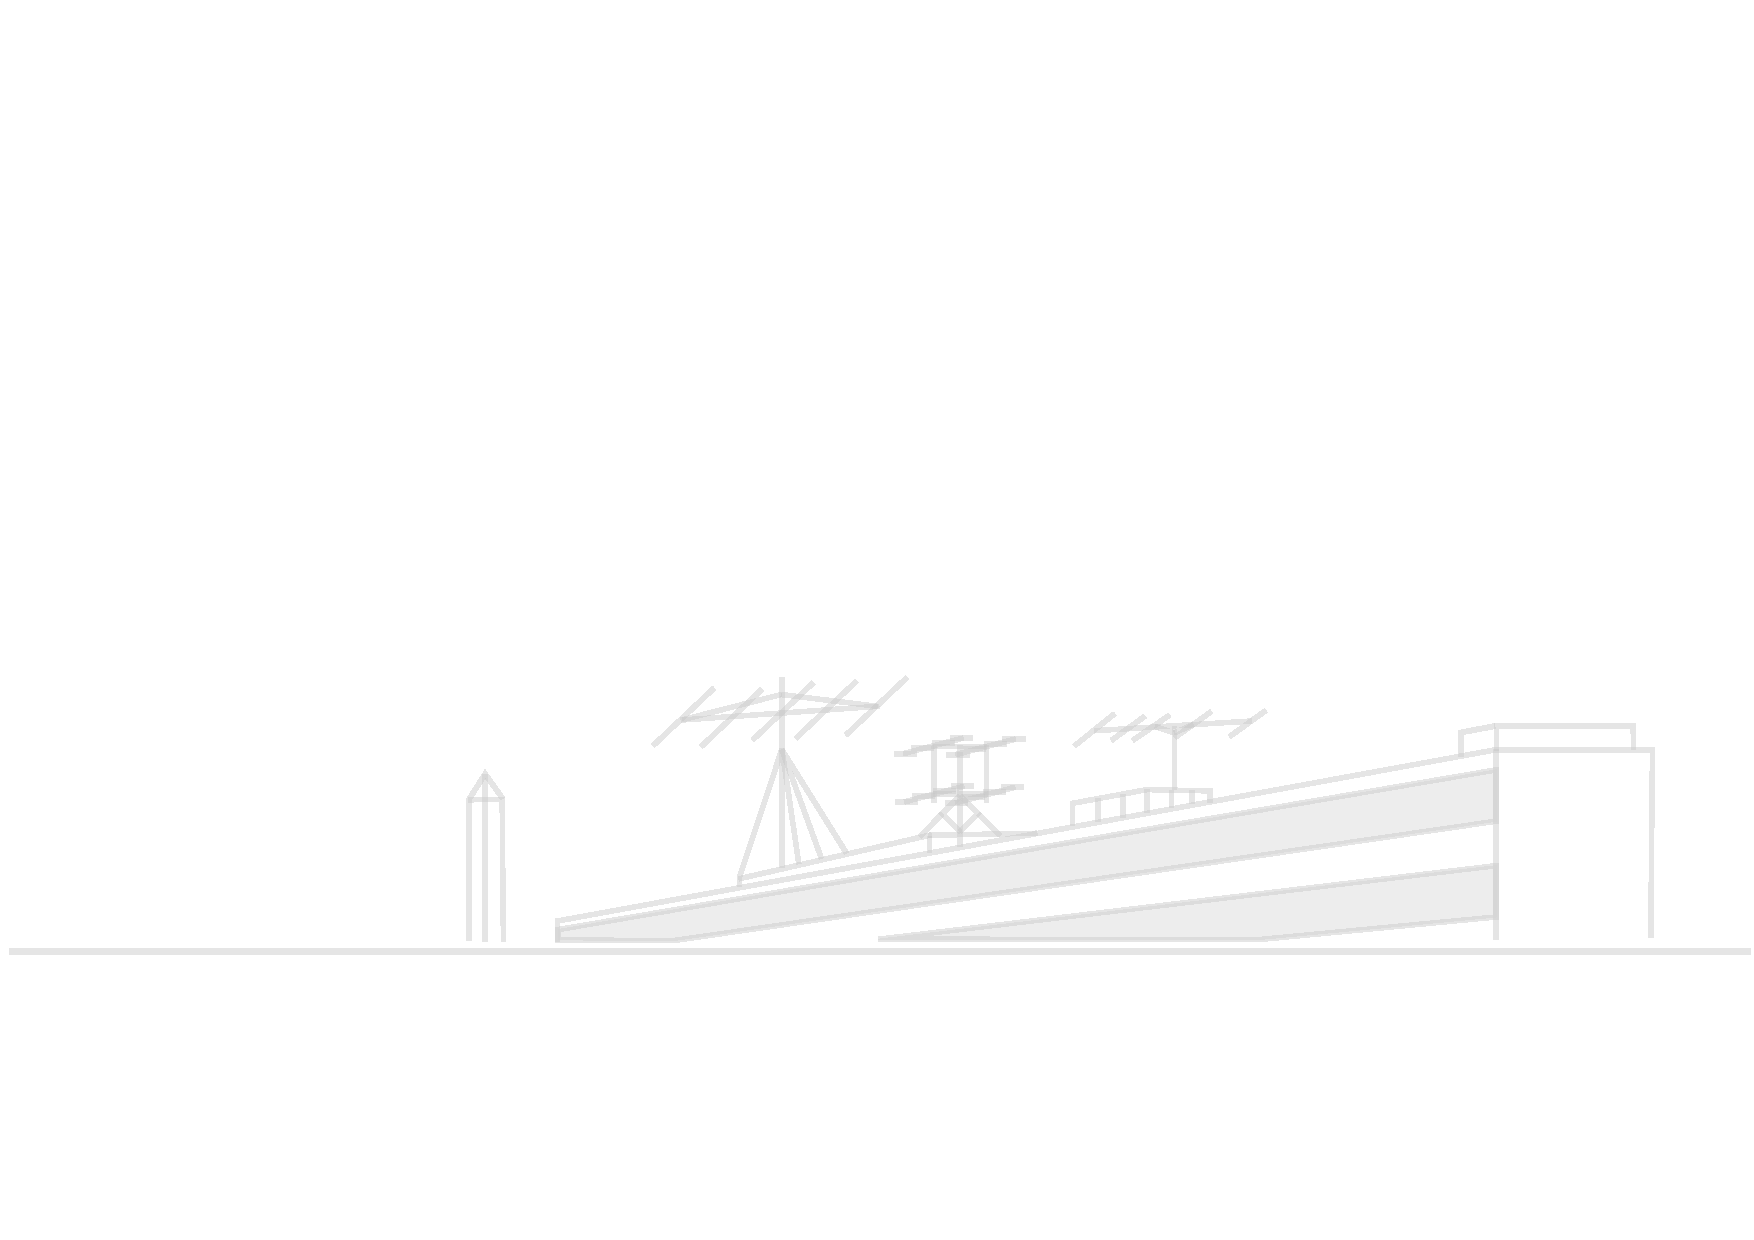
\includegraphics[width=17.8cm]{texdata/dk0tu_rooftop_background.pdf}
}

% Foliennummer einfügen
\setbeamertemplate{footline}[frame number]
%\setbeamertemplate{footline}{}

% Ändere das Zeichen vor jedem item
%\setbeamertemplate{itemize item}{\color{craneorange}$\blacktriangleright$}
%\setbeamertemplate{itemize subitem}{\color{craneorange}$\triangleright$}
%\setbeamertemplate{itemize subsubitem}{\color{craneorange}$\blacktriangleright$}

% Ändert die Blöcke 
\setbeamertemplate{blocks}[rounded][shadow=true]
% default | rounded [shadow=true|false]

%
% Eigene Kommandos
%

% Hack to get natbib and beamer working together. "The beamer user guide suggests
% that only the manual bibliography entry approach is supported"
% on some system it works out of the box, sometimes you need the hack :-(
% so check it --dl7bst
\ifdefined\newblock
    \relax
\else
    \newcommand{\newblock}{}
\fi

% \includedia command to generate png out of a dia file
% NEEDS installed dia and pdflatex option --shell-escape
\newcommand{\includedia}[1]{
    \immediate\write18{/usr/bin/dia #1.dia -e #1_diatmp.png -t png}
}

% RICHIG GROSSER FONT!
\newfont{\bigfont}{cmr10 at 144pt}
\newfont{\smallfont}{cmr10 at 8pt}

% Römische Ziffern
\makeatletter
\newcommand{\rmnum}[1]{\romannumeral #1}
\newcommand{\Rmnum}[1]{\expandafter\@slowromancap\romannumeral #1@}
\makeatother

% Schwarze Überschrift
%\setbeamercolor{frametitle}{fg=black}
%\setbeamercolor{title}{fg=black}

% Item- und Box-Farben
\definecolor{deepBlue}{HTML}{000066}
\setbeamercolor{itemize item}{fg=deepBlue}
\setbeamercolor{itemize subitem}{fg=deepBlue}
\setbeamercolor{description item}{fg=deepBlue}
\setbeamercolor{block title}{fg=deepBlue!100, bg=blue!15}
\setbeamercolor{block body}{fg=black, bg=blue!5}
\setbeamercolor{block title alerted}{fg=deepBlue, bg=red!75}
\setbeamercolor{block body alerted}{fg=black, bg=red!15}
\setbeamercolor*{block title example}{fg=blue!50, bg=blue!10}
\setbeamercolor*{block body example}{fg= blue, bg=blue!5}

%\setbeamercolor{section in head/foot}{parent=palette primary}
%\setbeamercolor{subsection in head/foot}{parent=palette secondary}
%\setbeamercolor{sidebar}{fg=darkblue,bg=yellow!90!orange}
%\setbeamercolor{title in sidebar}{fg=darkblue}
%\setbeamercolor{author in sidebar}{fg=darkblue}
%\setbeamercolor{section in sidebar}{fg=darkblue!10!black}
%\setbeamercolor{subsection in sidebar}{fg=darkblue!50!black}

% Titlepage Infos
\title{AFu-Kurs nach DJ4UF}
\author[DKØTU]{DKØTU\\ \footnotesize{Amateurfunkgruppe der TU Berlin}}
\institute[DKØTU]{\url{http://www.dk0tu.de} }

% PDF-Eigenschaften
\subject{DK0TU-Amateurfunkkurs nach DJ4UF}
\keywords{Amateurfunk Kurs HAM Radio Course CC-BY-NC-SA OpenSource TU Berlin DK0TU}

\subtitle{Technik Klasse E 07: \\
          Schwingkreise \& Filter \\[2em]}
\date{Stand 10.11.2015}
 \begin{document}

\begin{frame}
    \titlepage
    \vfill
    \begin{center}
        \ccbyncsaeu\\
        {\tiny This work is licensed under the \em{Creative Commons Attribution-NonCommercial-ShareAlike 3.0 License}.}\\[0.5ex]
         \tiny Amateurfunkgruppe der Technische Universität Berlin (AfuTUB), DKØTU
         %\includegraphics[scale=0.5]{img/DK0TU_Logo.pdf}
    \end{center}
\end{frame}


\section*{Schwingungs\-vorgang}
% TODO Tabelle

\begin{frame}
\frametitle{Schwingungen, wo gibt es denn sowas?}
	\begin{center}
		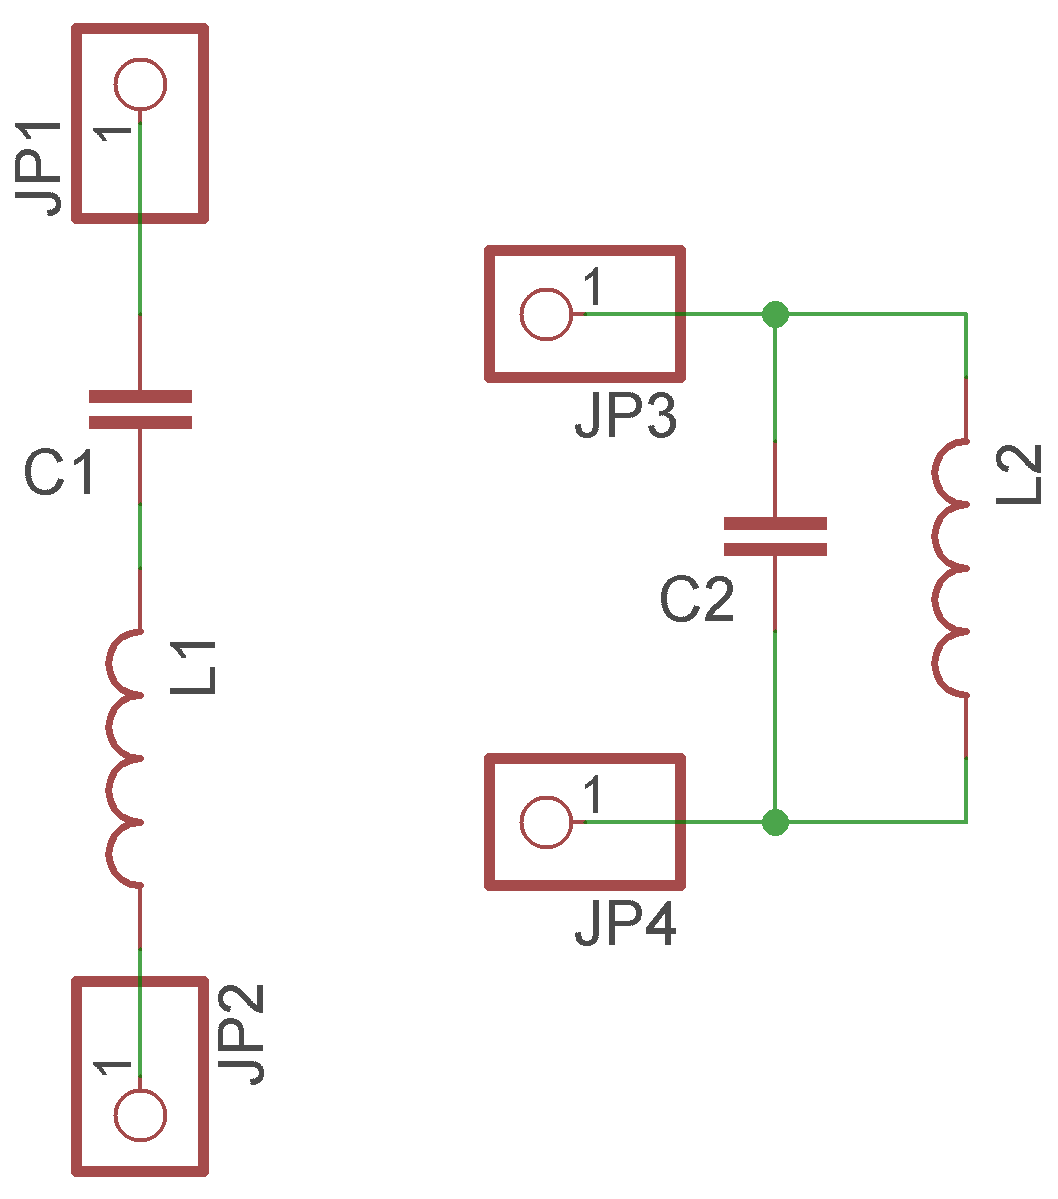
\includegraphics[width=\textwidth,height=.8\textheight,keepaspectratio]{e07/Schwingkreise.png}\\
		Abb.1: Reihen- \& Parallelschwingkreise
	\end{center}
\end{frame}

\begin{frame}
\frametitle{Reihenschwingkreis}
  \begin{columns}
    \column{0.37\textwidth}{
	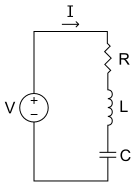
\includegraphics[width=1\textwidth]{e07/Serirenschw.png}\\
	\tiny{Abb: Reihenschwingkreis}
    }
    \column{0.62\textwidth}
    {      
    \begin{tabular}{l|llll}
        $f$ & $X_C$ & $X_L$ & $Z_g$ & $I_{ges}$ \\ \hline
		\hline
		$0$ & \only<1>{}\only<2>{$\infty$}\only<3>{$\infty$}  & \only<1>{}\only<2>{$0$}\only<3>{$0$} & \only<1>{}\only<2>{}\only<3>{$\infty$}  & \only<1>{}\only<2>{}\only<3>{$0$} \\
		$\infty$ & \only<1>{}\only<2>{$0$}\only<3>{$0$}   & \only<1>{}\only<2>{$\infty$}\only<3>{$\infty$} & \only<1>{}\only<2>{}\only<3>{$\infty$} & \only<1>{}\only<2>{}\only<3>{$0$}  \\
		$f_{res}$  & \only<1>{}\only<2>{$\frac{1}{j \omega C} =$}\only<3>{$\frac{1}{j \omega C} =$} & \only<1>{}\only<2>{$j \omega L$}\only<3>{$j \omega L$}  & \only<1>{}\only<2>{}\only<3>{Min}  & \only<1>{}\only<2>{}\only<3>{Max} \\
	\end{tabular}
    }
    \end{columns}
\end{frame}

\begin{frame}
\frametitle{Parallelschwingkreis}
  \begin{columns}
    \column{0.37\textwidth}{
		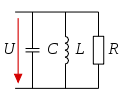
\includegraphics[width=1\textwidth]{e07/Parallelschw.png}\\
		\tiny{Abb: Parallelschwingkreis}
    }
    \column{0.62\textwidth}
    {      
    \begin{tabular}{l|llll}
        $f$ & $X_C$ & $X_L$ & $Z_g$ & $I_{ges}$ \\ \hline
		\hline
		$0$ & \only<1>{}\only<2>{$\infty$}\only<3>{$\infty$}  & \only<1>{}\only<2>{$0$}\only<3>{$0$} & \only<1>{}\only<2>{}\only<3>{$0$}  & \only<1>{}\only<2>{}\only<3>{Max} \\
		$\infty$ & \only<1>{}\only<2>{$0$}\only<3>{$0$}   & \only<1>{}\only<2>{$\infty$}\only<3>{$\infty$} & \only<1>{}\only<2>{}\only<3>{$0$} & \only<1>{}\only<2>{}\only<3>{Max}  \\
		$f_{res}$  & \only<1>{}\only<2>{$\frac{1}{j \omega C} =$}\only<3>{$\frac{1}{j \omega C} =$} & \only<1>{}\only<2>{$j \omega L$}\only<3>{$j \omega L$}  & \only<1>{}\only<2>{}\only<3>{Max}  & \only<1>{}\only<2>{}\only<3>{Min} \\
	\end{tabular}
   }
   \end{columns}
\end{frame}

\begin{frame}
\frametitle{Aber warum schwingt das denn jetzt?}
\begin{center}
	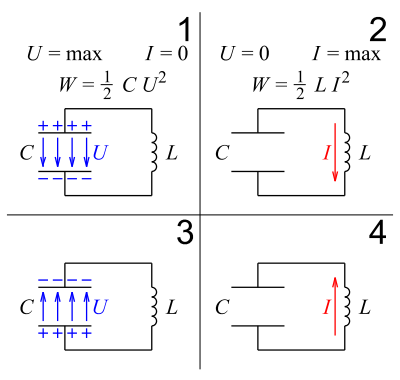
\includegraphics[width=.8\textwidth,height=.8\textheight,keepaspectratio]{e07/Schwingkreis.png}\\
	Abb.2: Energie in einem LC-Schwingkreis \cite{wmde} \\
\end{center}
\end{frame}

\begin{frame}
  % XXX klappt nur in bestimmten PDF Readern
  \begin{center}
 % \animategraphics[loop,width=\textwidth,height=.85\textheight,keepaspectratio,controls]{2}{e07/Tuned_circuit_animation_3-}{0}{11}
  \tiny{animierte Darstellung (\url{http://en.wikipedia.org/wiki/File:Tuned_circuit_animation_3.gif})}
  \end{center}
\end{frame}

\begin{frame}
\frametitle{Schwingung in der Realität?}
    \begin{center}
	    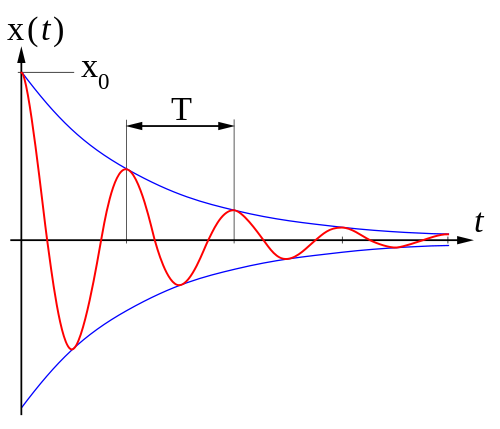
\includegraphics[width=.8\textwidth,height=.8\textheight,keepaspectratio]{e07/Damped_oscillation_graph.png}\\
	    Abb: Gedämpfte Schwingung \\
    \end{center}
    \begin{block}{\"Ubung}
        Wodurch wird die Schwingung gedämpft? \\ Was müsste getan werden um die Schwingung aufrecht zu erhalten?
    \end{block}
\end{frame}

\begin{frame}
\frametitle{Resonanzfrequenz}
\begin{center}
  \begin{block}{Frequenz mit der sich die Schwingung wiederholt}
	\Huge{$ f_{res} = \cfrac{1}{2 \cdot \pi \cdot \sqrt{L \cdot C}} $}
  \end{block}
  \pause
  Durch Verluste (insbesondere Widerstand) kommt es zur gedämpften Schwingung.
\end{center}
\end{frame}

\section*{Reihen\-schwing\-kreis}
\begin{frame}
\frametitle{Reihenschwingkreis}
\begin{center}
	\begin{minipage}{0.4\textwidth}
	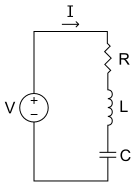
\includegraphics[width=\textwidth,height=.5\textheight,keepaspectratio]{e07/Serirenschw.png}\\
	\tiny{Abb.3: Reihenschwingkreis \cite{wmen}}
	\end{minipage}
	\begin{minipage}{0.4\textwidth}
	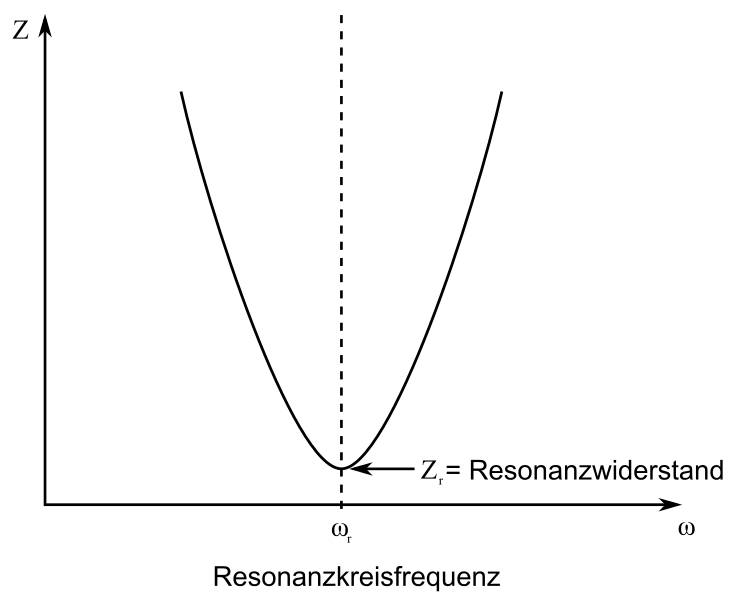
\includegraphics[width=\textwidth,height=.5\textheight,keepaspectratio]{e07/SerirenschwSig.png}\\
	\tiny{Abb.4: Resonanzwiderstand \cite{wmen}} 
	\end{minipage}
\end{center}
\begin{itemize}
	\item Im Verlauf der Frequenzänderung ändert sich der Gesamtwellenwiderstand $Z$ des Schwingkreises
	\item Der Schwingkreis hat als minimale Impedanz seinen ohmschen Wert, da sich bei der Resonanzfrequenz $f_R$ die induktiven und kapazitiven Anteile gegenseitig aufheben
\end{itemize}
\end{frame}

\section*{Parallel\-schwing\-kreis}
\begin{frame}
\frametitle{Parallelschwingkreis}
\begin{center}
	\begin{minipage}{0.4\textwidth}
	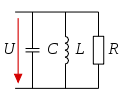
\includegraphics[width=\textwidth,height=.5\textheight,keepaspectratio]{e07/Parallelschw.png}\\
	\tiny{Abb.5: Parallelschwingkreis \cite{wmen}}
	\end{minipage}
	\begin{minipage}{0.4\textwidth}
	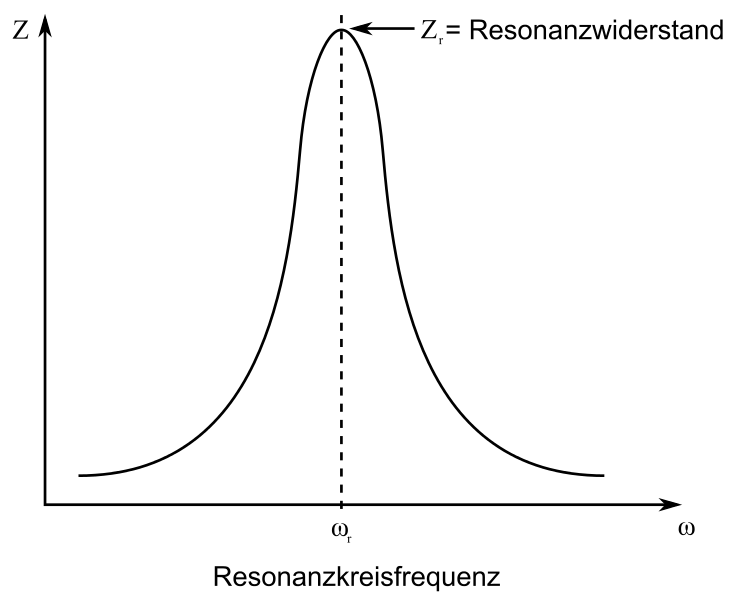
\includegraphics[width=\textwidth,height=.5\textheight,keepaspectratio]{e07/ParallelschwSig.png}\\
	\tiny{Abb.6: Resonanzwiderstand \cite{wmen}} 
	\end{minipage}
\end{center}
\begin{itemize}
	\item Der Parallelschwingkreis verhält sich genau entgegen gesetzt zum Reihenschwingkreis
	\item Dieser zeigt bei niedrigen und hohen Frequenzen das Verhalten eines Leiters
	\item Bei der Resonanzfrequenz hingegen steigt der Wellenwiderstand an, da hier nur noch der ohmsche Widerstand wirkt
\end{itemize}
\end{frame}



\section*{Filter}
\subsection*{Saugkreis}
\begin{frame}
  \frametitle{Saugkreis}
  \begin{center}
    % https://upload.wikimedia.org/wikipedia/commons/c/c9/Saugkreis.png
    \includegraphics<1>[width=\textwidth,height=.5\textheight,keepaspectratio]{e07/Saugkreis.png}
    \includegraphics<2>[width=\textwidth,height=.5\textheight,keepaspectratio]{e07/SerirenschwSig.png}
  \end{center}
  \pause
  \begin{itemize}
    \item vor und nach der Resonanzfrequenz hoher Widerstand
    \item nur Wechselspannungen mit Frequenzen in der Nähe der Resoanzfrequenz werden durchgelassen
    \item Anwendung: Audiotechnik
  \end{itemize}
\end{frame}

\subsection*{Sperrkreis}
\begin{frame}
  \frametitle{Sperrkreis}
  \begin{center}
    % https://upload.wikimedia.org/wikipedia/commons/e/ef/Sperrkreis.png
    \includegraphics<1>[width=\textwidth,height=.5\textheight,keepaspectratio]{e07/Sperrkreis.png}
    \includegraphics<2>[width=\textwidth,height=.5\textheight,keepaspectratio]{e07/ParallelschwSig.png}
  \end{center}
  \pause
  \begin{itemize}
    \item bei der Resonanzfrequenz hoher Widerstand
    \item die Resonanzfrequenz wird gefiltert
    \item Anwendungen: Mehrbandantennen; Filtern von starken Sendern
  \end{itemize}
\end{frame}

\subsection*{Tiefpass}
\begin{frame}
\frametitle{Tiefpass}
\begin{center}
	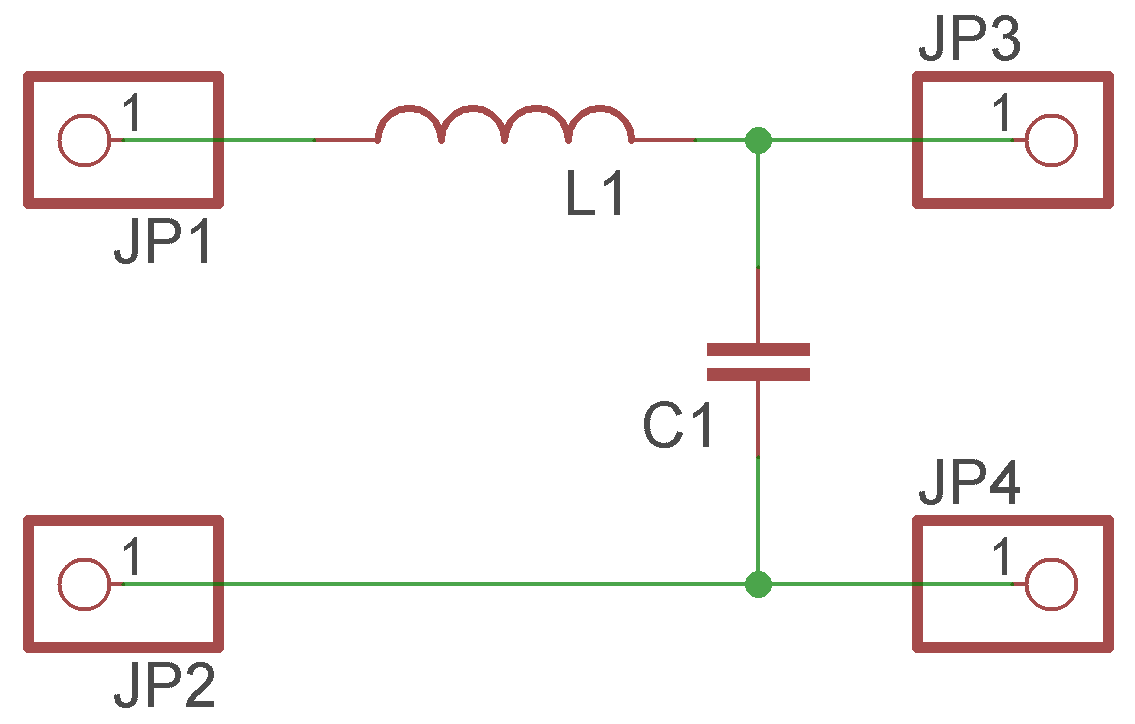
\includegraphics[width=\textwidth,height=.5\textheight,keepaspectratio]{e07/LC-Tiefpass.png}\\
	Abb.8: LC-Tiefpass
\end{center}
\begin{itemize}
	\item Bei steigender Frequenz sinkt der Blindwiderstand $X_L$ und der Blindwiderstand $X_C$ steigt
	\item Bei sinkender Frequenz hingegen steigt $X_L$ und $X_C$ sinkt
	\item Dadurch werden nur niedrige Frequenzen durchgelassen 
\end{itemize}
\end{frame}

\subsection*{Hochpass}
\begin{frame}
\frametitle{Hochpass}
\begin{center}
	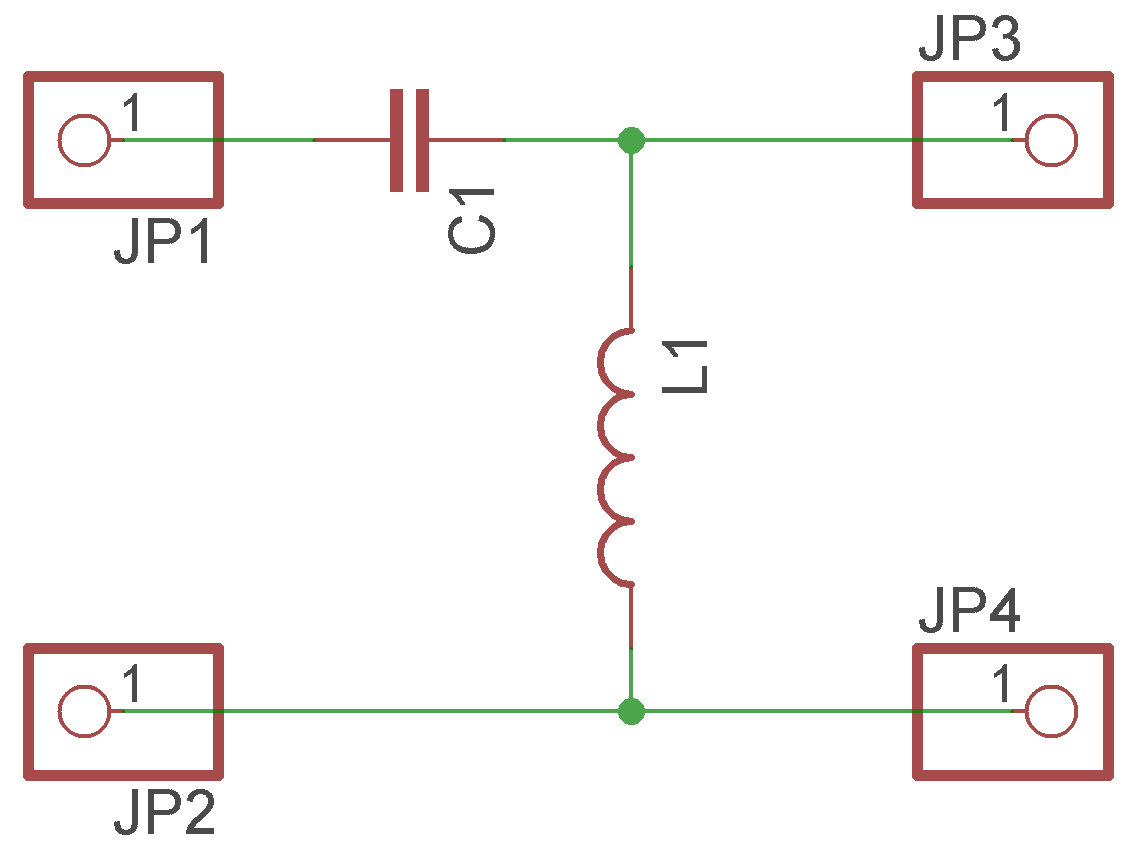
\includegraphics[width=\textwidth,height=.5\textheight,keepaspectratio]{e07/LC-Hochpass.png}\\
	Abb.9: LC-Hochpass
\end{center}
\begin{itemize}
	\item Bei steigender Frequenz steigt der Blindwiderstand $X_L$ und der Blindwiderstand $X_C$ sinkt
	\item Bei sinkender Frequenz hingegen sinkt $X_L$ und $X_C$ steigt
	\item Dadurch werden nur hohe Frequenzen durchgelassen 
\end{itemize}
\end{frame}


\section*{Referenzen}

\renewcommand{\refname}{Referenzen}

\hypertarget{refs}{}
\textcolor{white}{} \\ %\vspace{} geht nicht
\Large Referenzen/Links
\footnotesize

\begin{thebibliography}{}
    \bibitem{e03}   Moltrecht E 07: \\
                    \url{http://www.darc.de/referate/ajw/ausbildung/darc-online-lehrgang/technik-klasse-e/technik-e07/}
    \bibitem{wp}    Wikipedia DE: \\
                    \url{http://de.wikipedia.org/wiki/Ohmsches_Gesetz}\\ 
                    \url{http://de.wikipedia.org/wiki/Elektrische_Leistung}\\ 
                    \url{http://de.wikipedia.org/wiki/lektrische_Energie#Elektrische_Energie_in_einem_elektrischen_Feld}\\ 
    \bibitem{wmde}	Wikimedia DE:\\
    				\url{http://commons.wikimedia.org/wiki/File:LC_circuit_4_times_new_version.svg?uselang=de}\\
   	\bibitem{wmen}	Wikimedia EN:\\
   					\url{http://en.wikipedia.org/wiki/File:Tuned_circuit_animation_3.gif}\\
   					\url{http://commons.wikimedia.org/wiki/File:RLC_series_circuit_v1.svg}\\
   					\url{http://commons.wikimedia.org/wiki/File:Resonanzwiderstand_serie.svg}\\
   					\url{http://commons.wikimedia.org/wiki/File:KondiSpuleWiderstandParallel.svg}\\
   					\url{http://commons.wikimedia.org/wiki/File:Resonanzwiderstand_parallel.svg}\\
   					\url{http://commons.wikimedia.org/wiki/File:Bandlimited_3dB_LP.svg}\\
   					
\end{thebibliography}

% Hier könnte noch eine Kontaktfolie stehen

\end{document}

